%\documentclass[times, 11pt, onecolumn]{article} 
%\documentclass[times, 10pt]{article} 
%\documentclass{article} 

\documentclass[conference,final]{IEEEtran}

\usepackage{latex8}
\usepackage{times}

\usepackage[utf8]{inputenc}
\usepackage{graphicx}
\usepackage{url}
\usepackage{float}
\usepackage{times}    
\usepackage{multirow}    
\usepackage{listings}   
\usepackage{times}     
\usepackage{paralist}    
\usepackage{wrapfig}    
\usepackage[small,it]{caption}
\usepackage{multirow}
\usepackage{ifpdf}
\usepackage{subfigure}

\usepackage{listings}
\usepackage{keyval}  
\usepackage{color}
\definecolor{listinggray}{gray}{0.95}
\definecolor{darkgray}{gray}{0.7}
\definecolor{commentgreen}{rgb}{0, 0.4, 0}
\definecolor{darkblue}{rgb}{0, 0, 0.4}
\definecolor{middleblue}{rgb}{0, 0, 0.7}
\definecolor{darkred}{rgb}{0.4, 0, 0}
\definecolor{brown}{rgb}{0.5, 0.5, 0}

\lstdefinestyle{myListing}{
  frame=single,   
  backgroundcolor=\color{listinggray},  
  %float=t,
  language=C,       
  basicstyle=\ttfamily \footnotesize,
  breakautoindent=true,
  breaklines=true
  tabsize=2,
  captionpos=b,  
  aboveskip=0em,
  belowskip=-2em,
  %numbers=left, 
  %numberstyle=\tiny
}      

\lstdefinestyle{myPythonListing}{
  frame=single,   
  backgroundcolor=\color{listinggray},  
  %float=t,
  language=Python,       
  basicstyle=\ttfamily \footnotesize,
  breakautoindent=true,
  breaklines=true
  tabsize=2,
  captionpos=b,  
  %numbers=left, 
  %numberstyle=\tiny
}

\newcommand{\up}{\vspace*{-1em}}
\newcommand{\upp}{\vspace*{-0.5em}}


\title{
  ~\\[-3em]
  Developing Applications With Loosely-Coupled Sub-Tasks Using a
  Standard Programmatic Interface}

  \author{
    ~\\[-2em]
    % Unsure of Author List$^{1}$ \\
    Shantenu Jha$^{1,2,3}$, Joohyun Kim$^{1}$,
    Yaakoub El-Khamra$^{1}$, Andre Lukow, \\ 
    Hartmut Kaiser$^{1}$ and Andre Merzky$^{1}$ \\
    \small{\emph{$^{1}$Center for Computation \& Technology, Louisiana State University, USA}}\\
    \small{\emph{$^{2}$Department of Computer Science, Louisiana State
        University, USA}}\\
    \small{\emph{$^{3}$e-Science Institute, Edinburgh, UK}}\\
  }

%\date{}



\def\acknowledgementname{Acknowledgements}

\newenvironment{acknowledgement}%

{\section*{\acknowledgementname}%
\parindent=0pt%
}

\newif\ifdraft
\drafttrue
\ifdraft
\newcommand{\kimnote}[1]{ {\textcolor{green} { ***JK: #1 }}}
\newcommand{\alnote}[1]{ {\textcolor{blue} { ***AL: #1 }}}
\newcommand{\amnote}[1]{ {\textcolor{magenta} { ***AM: #1 }}}
\newcommand{\jhanote}[1]{ {\textcolor{red} { ***SJ: #1 }}}
\else
\newcommand{\kimnote}[1]{}
\newcommand{\alnote}[1]{}
\newcommand{\amnote}[1]{}
\newcommand{\jhanote}[1]{}
\fi

\begin{document} 


\maketitle    

\begin{abstract}
  The Simple API for Grid Applications (SAGA) can be used to
  programmatically develop a very wide-range of distributed
  applications.  In this paper we describe how SAGA has been used to
  develop two different applications from the following classes of
  distributed applications (i) applications based upon the loosely
  coupled of homogenous sub-tasks and, (ii) applications based upon
  loosely coupled simulations of heterogenous sub-tasks. The specific
  applications developed are Replica-Exchange simulations using
  Molecular Dynamics and Kalman-Filter based application for reservoir
  simulation.  We briefly discuss the specific applications developed
  and the typical science problems tackled using these applications.
  We will describe the application characteristics of the two
  case-studies, with a focus on the distributed logic of these
  simulations, and not the core simulation logic of the applications.
  The paper analyses and contrasts the application characteristics of
  the examples, and shows how they are supported using SAGA, often in
  conjunction with other programming frameworks such as Cactus.  The
  primary aim of this paper is to demonstrate how SAGA can be an
  effective tool for programmatically representing and implemeting the
  logic of coordination and orchestrating multiple, distributed tasks,
  while remaining agnostic to the actual mechanism, ie. details of the
  distributed environment. We will highlight the importance of
  programming abstractions and how frameworks that provide common
  programming patterns can be used to simplify the construction of
  distributed applications.
\end{abstract}


The story is as follows. 

We have two distinct applications -- REMD and a Kalman-Filter based
applications.

These applications are prototypes of two important applications
classes -- loosely coupled multiple identical sub-tasks (ie replicas)
and multiple, loosely-coupled but heterogenous sub-tasks.  (In the
latter case, they are not only heterogenous they are also highly
irregular).  We have demonstrated that these applications work
perfectly well in distributed environments.

The aim of this paper is to demonstrate that these applications can be
deployed and executed on the high-end machine (actually highest-end
machine available to the academic community) using exactly the same
framework, ie, there exists a standard, programmatic approach to
codify these applications such that they can be seamlessly run on any
underlying infrastructure. Critically this implies that the the
application developer focusses on supporting the application
characteristics and not worrying about the details of the underlying
infrastructure.

Although both are classified as loosely-coupled, the nature of the
coupling between the sub-tasks varies. In the former, the sub-tasks
progress independent of other sub-tasks with the exception of one
(referred to as the paired replica). There is a pair-wise exchange of
some parameters after a certain time-period (maybe fixed or not), and
it is possible that the paired-replicas differ, i.e., a replica is
paired with a different replica as time progresses. If the sub-task
that a replica is paired with is not is not ready for exchange, the
sub-tasks goes into a wait state, i.e., the consequence of
load-balancing is typically localized to the paired replica. If there
are multiple replicas in a wait state, sophisticated scheduling can be
invoked to progress waiting tasks. \jhanote{elaborate a bit}

It is important to contrast this ``coupling'' with the coupling in the
latter application's (Kalman Filter) case. For the Kalman-Filter
application, the multiple sub-tasks need to {\it all} complete
as there is a global synchronization point, and the output
of all sub-tasks are required to generate the input for the next
stage.

It is important to appreciate the nature of the coupling of
the sub-tasks, as it imposes constraints on the 
(i) scheduling strategies, (ii) speculative computing (iii) resource
mapping strategies.


\jhanote{The bulk of the next three sections should be pretty much 
  a cut and paste job. What is really required is i. run the
  multi-tasks of the kalman filter  application entirely on Ranger
  ii. run the multi-tasks of the replica exchange entirely on 
  ranger}

\section{SAGA: A Standard Programming Interface}


\begin{figure}[!h]
  \begin{center}
    \subfigure{\label{sagalayer1}
      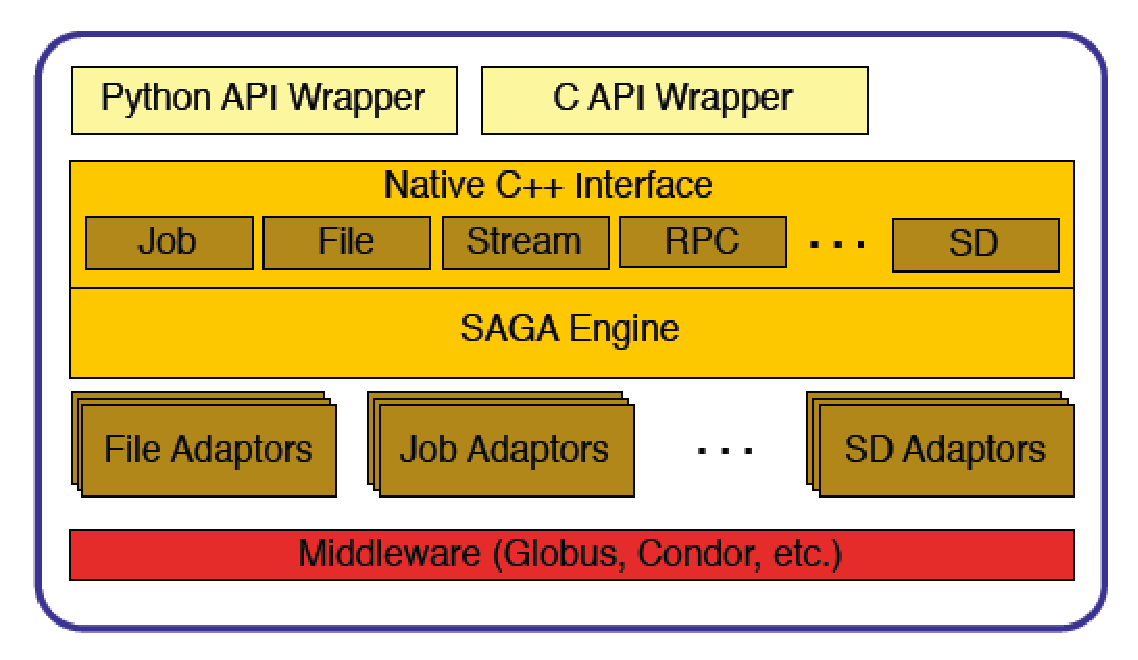
\includegraphics[width=3.55in]{saga_layered_landscape}}     
%     \subfigure{\label{sagalayer2}
%       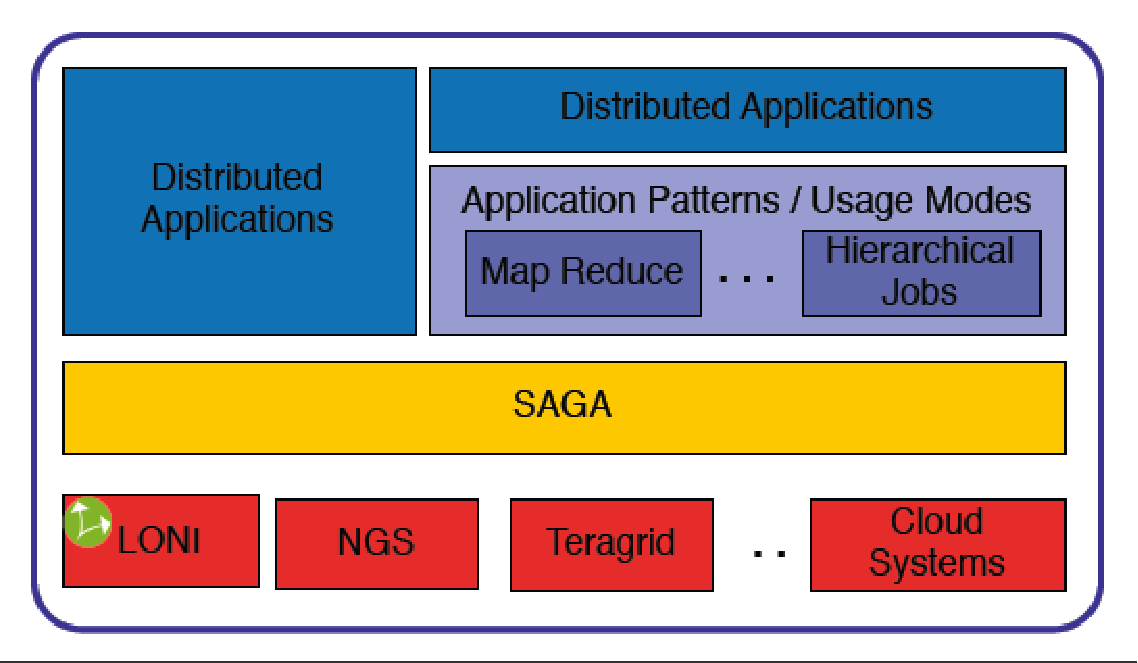
\includegraphics[width=3.55in]{saga_layered_application}}
  \end{center}
  \caption{Layered schematic of the different components of the SAGA
    landscape.  Middleware specific adaptors applications developed
    using SAGA make applications developed using SAGA grid
    portable. Schematic showing the different ways in which SAGA can
    be used to develop distributed applic ations}
 \label{sagalayer}
\end{figure}


\begin{figure}[!h]
  \begin{center}
%     \subfigure{\label{sagalayer1}
%       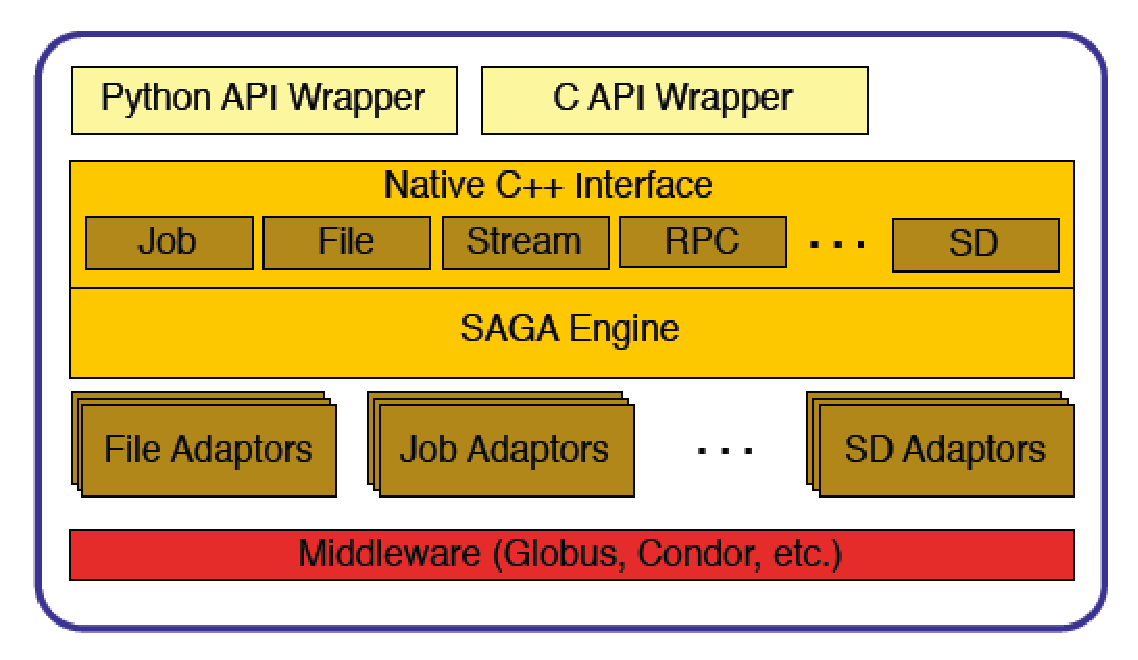
\includegraphics[width=3.55in]{saga_layered_landscape}}     
    \subfigure{\label{sagalayer2}
      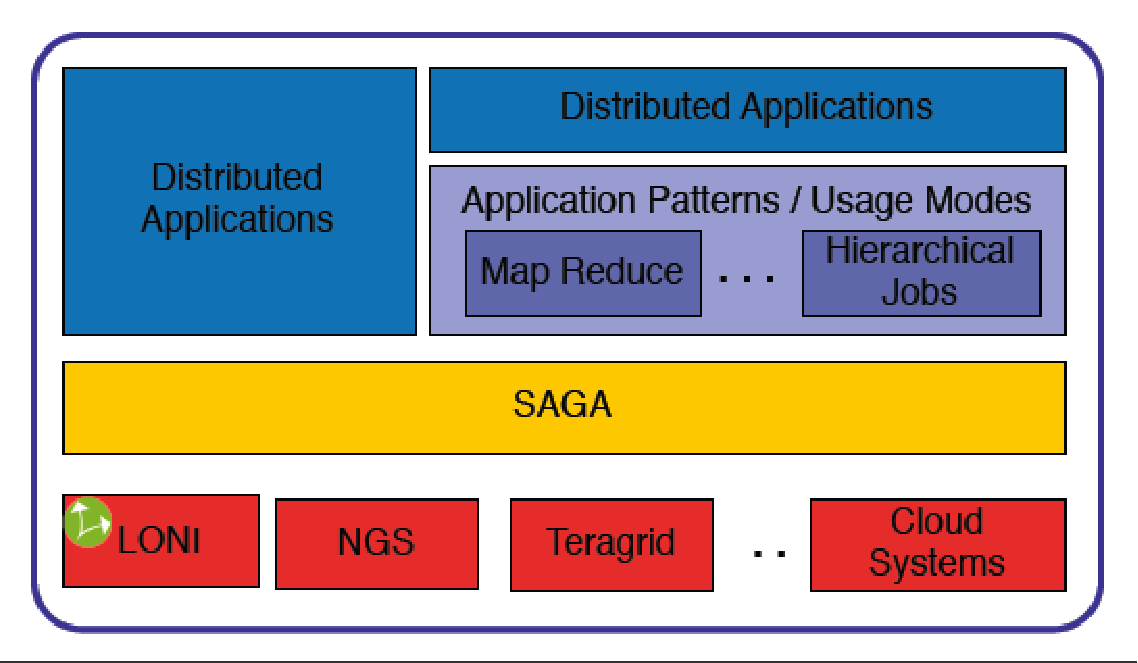
\includegraphics[width=3.55in]{saga_layered_application}}
  \end{center}
  \caption{Layered schematic of the different components of the SAGA
    landscape.  Middleware specific adaptors applications developed
    using SAGA make applications developed using SAGA grid
    portable. Schematic showing the different ways in which SAGA can
    be used to develop distributed applic ations}
 \label{sagalayer}
\end{figure}


\section{Application With Multiple Loosely-Coupled Homogenous
  Sub-Tasks}

\subsection{Application Description}

\subsection{Application Architecture}

\subsection{Deploying on Distributed Resources}

\subsection{Deploying on Ranger}


\section{Applications With Multiple Loosely-Coupled Heterogenous
  Sub-Tasks}

\subsection{Application Description}

\subsection{SAGA and Cactus: A Powerful Application Development
  Framework}

\subsection{Deploying on Distributed Resources}

\subsection{Deploying on Ranger}

BQP used for the first time to dynamically determine queue and model
size within a given system to submit sub-task to...


\section{Any Other Applications}

 -- Data parallel applications

\section{Take Home Message}

\begin{itemize}
\item  SAGA provides the ability to create multi-tasks applications that
  can exploit multiple and different infrastructure types.

\item Not only do we need support for different programming models, 
this is also proof of support for agile execution models.

\item We have demonstrated this via the implementation of two
  different applications and running them in two very different
  execution environments.
\end{itemize}







% \Section{Introduction}
%   There exist several applications which require several smaller but
%   heterogenous tasks to be solved in multiple-stages as part of the
%   overall solution.  Often the time-to-solution is the single most
%   important metric.  Distributed resources can thus help, especially
%   when combined with opportunistic scheduling/execution.  However, the
%   desire/need to use distributed computing comes with its own/unique
%   set of challenges.
  
%   We discuss three application types that are in turn composed of
%   multiple, smaller but {\it loosely-coupled} tasks -- Replica
%   Dynamics, Satisfiability problems, and Kalman filtering
%   applications.  Although these applications types are similar in that
%   they are comprised of multiple, smaller tasks, they are different in
%   that the individual sub-tasks are dissimilar for different reasons.
  
%   These application types are often multi-staged, with varying levels
%   of dependency between the stages. There could be, strict ordering
%   between the stages, ie. if all tasks in a stage must complete and be
%   globally synchronised before the next stage can begin. Thus there is
%   coupling between tasks within a given stage, and there is coupling
%   between stages.

%   Other challenges that any many-task system will encounter are: (i)
%   scheduling these sub-tasks is a challenge, (ii) level of speculative
%   computing that can be employed.

%   In parallel replica dynamics, the replicas can run for different
%   time durations between different stages. In replica-exchange
%   dynamics, the number and frequency of exchanges can vary.  Different
%   stages of this application vary; in other words, there is
%   time-domain heterogenity.

%   In Kalman filter based applications, the number and size of 
%   tasks between different stages varies. 

%   In the general class of satisfiability-based applications, as well
%   as the learning-based algorithms, there are elements of both kinds
%   of heterogenity between stages. GridSAT is an interesting example.
         
\newpage
                  
\section*{Acknowledgement}
This work would not have been possible without the efforts and support
of the wider SAGA team. Important funding for SAGA specification and
development has been provided by the UK EPSRC grant number
GR/D0766171/1 (via OMII).  SJ acknowledges the e-Science Institute,
Edinburgh for supporting the research theme, ``Distributed Programming
Abstractions''.  This work has also been made possible thanks to the
internal resources of the Center for Computation \& Technology (CCT)
at Louisiana State University and computer resources provided by LONI.


\bibliographystyle{IEEEtran}
\bibliography{saga}
\end{document}


